\chapter{Discrete Circuitry Design}
This chapter contains the discrete circuit which has been briefly reviewed in section \ref{section:SF}.
We build this circuit to practice the constant current method.

\section{Transforming the design from p-type measuring into n-type measuring}
In \cite{SF1}, the circuit is for p-type ISFET element (Fig.\ref{fig:SF_schematic_old}).
Our nanowire element is n-type.
Hence we transform the circuit as Fig.\ref{fig:SF_schematic}.
\begin{figure}[!htbp]
    \centering
    \includegraphics[width=0.8\textwidth] {../images/chapter4/SFdiscrete_old.png}
    \caption{The schematic of read-out circuit from \cite{SF1}. The ISFET is a p-type element. It is controlled by the current source $I_b$ whose sub-circuit is shown at right.}
    \label{fig:SF_schematic_old}
\end{figure}
\begin{figure}[!htbp]
    \centering
    \includegraphics[width=0.8\textwidth] {../images/chapter4/SFdiscrete_schematic.png}
    \caption{The our circuit schematic transformed from Fig.\ref{SF_schematic_old}. The center transistor is a n-type element. It is controlled by the current source $I_b$ whose sub-circuit is shown at right.}
    \label{fig:SF_schematic}
\end{figure}


\section{Circuit Description}
The circuit is divided into two sections: the circuit body and the biasing current source (Ib).

\subsection*{Circuit Body}
The circuit body section is a source follower structure.
The input of the circuit is at the floating gate ($G$) of the center transistor, where the output is at its source ($S$).

The $I_D$ of the transistor is controlled by the Ib.
The leakage current flowing into the negative input of OP2 is less than 0.1nA.
Thus the $I_D$ of the transistor should always be same as bias current $I_b$.

The $V_{DS}$ is always equal to the potential difference ($I_0 \times R_0$) across the resistor $R_0$.
This is achieved by two OP-based unity gain buffer.
They connected serially with $R_b$ and cause the voltage at drain end $D$ follows the voltage at $S$.


\subsection*{biasing current source (Ib)}
The Ib is in fact a current scale down circuit.
By concerning the OP as ideal, the node $OP+$ has the same voltage with $OP-$.
This equalize the potential difference across two resistors whose resistance are different by $N$-fold.
As the result, the current of Ib and Is are also different by $N$-fold.
$I_b = I_s / N$.

The capacitor is for filtering. It filter the high frequency noise out to create a stable output current.


\section{Discrete Element}
We use tlc2264 made by Texas Instrument (TI) as our OP.
This OP element has working voltage of $\pm 5v$ and can perform rail-to-rail output operation.
Its gain (Large-signal differential voltage amplification rate) is 170 for the output load greater than 50k.

For the current source Is and I0, we use lm334 made by National Semiconductor.
It is a 3-terminal adjustable current sources with wide dynamic voltage range of 1v to 40v and current accuracy of $\pm 3\%$.
In out experiment, the current $I_s$ is fixed at $1\mu A$ where its output impedance is $1.2G\Omega$.

\section{Circuit Performance and Conclusion}
We examined the performance of our circuit by plotting its $I_D$-$V_G$ curve.
The $I_0$, $R_0$ and $V_G$ were kept constant.
We swept the $I_D$ by changing the $N$ value with a variable resistor.
The $N$ ranges from 1 to 1000.
And the Ib circuit should produces bias current $I_b$ from $1\mu A$ to $1n A$.

We measured the output voltage at $S$ and subtracted this value from $V_G$ to get the respective $V_{GS}$.
These two value gave result to the $I_D$-$V_G$ curve in Fig.\ref{fig:SF_result}.

The measurement result shows that when $I_D$ is larger than $10n A$, the circuit is functional.
The $I_D$-$V_G$ curve obtained by the circuit is same as the one obtained by directly sweeping $V_G$ and measuring $I_D$ with Source Meter (Keithley 2602).

The circuit fails when $I_D$ is smaller than $10n A$.
This is caused by the unmatched impedance, which we have discussed in section.\ref{section:SF}.

The output impedance of Ib circuit is:
\begin{equation} \label{eq:rcs2_again}
    N\times R_s
\end{equation}
$R_s$ is the output impedance of current source Is which equals to $1.2G\Omega$.
And the input impedance of transistor is:
\begin{equation} \label{eq:rsf2_again}
    \frac{1}{g_m}
\end{equation}

We plot the $I_D$-Impedance plot in Fig.\ref{fig:SF_imp}.


 \begin{figure}[!htbp]
    \centering
    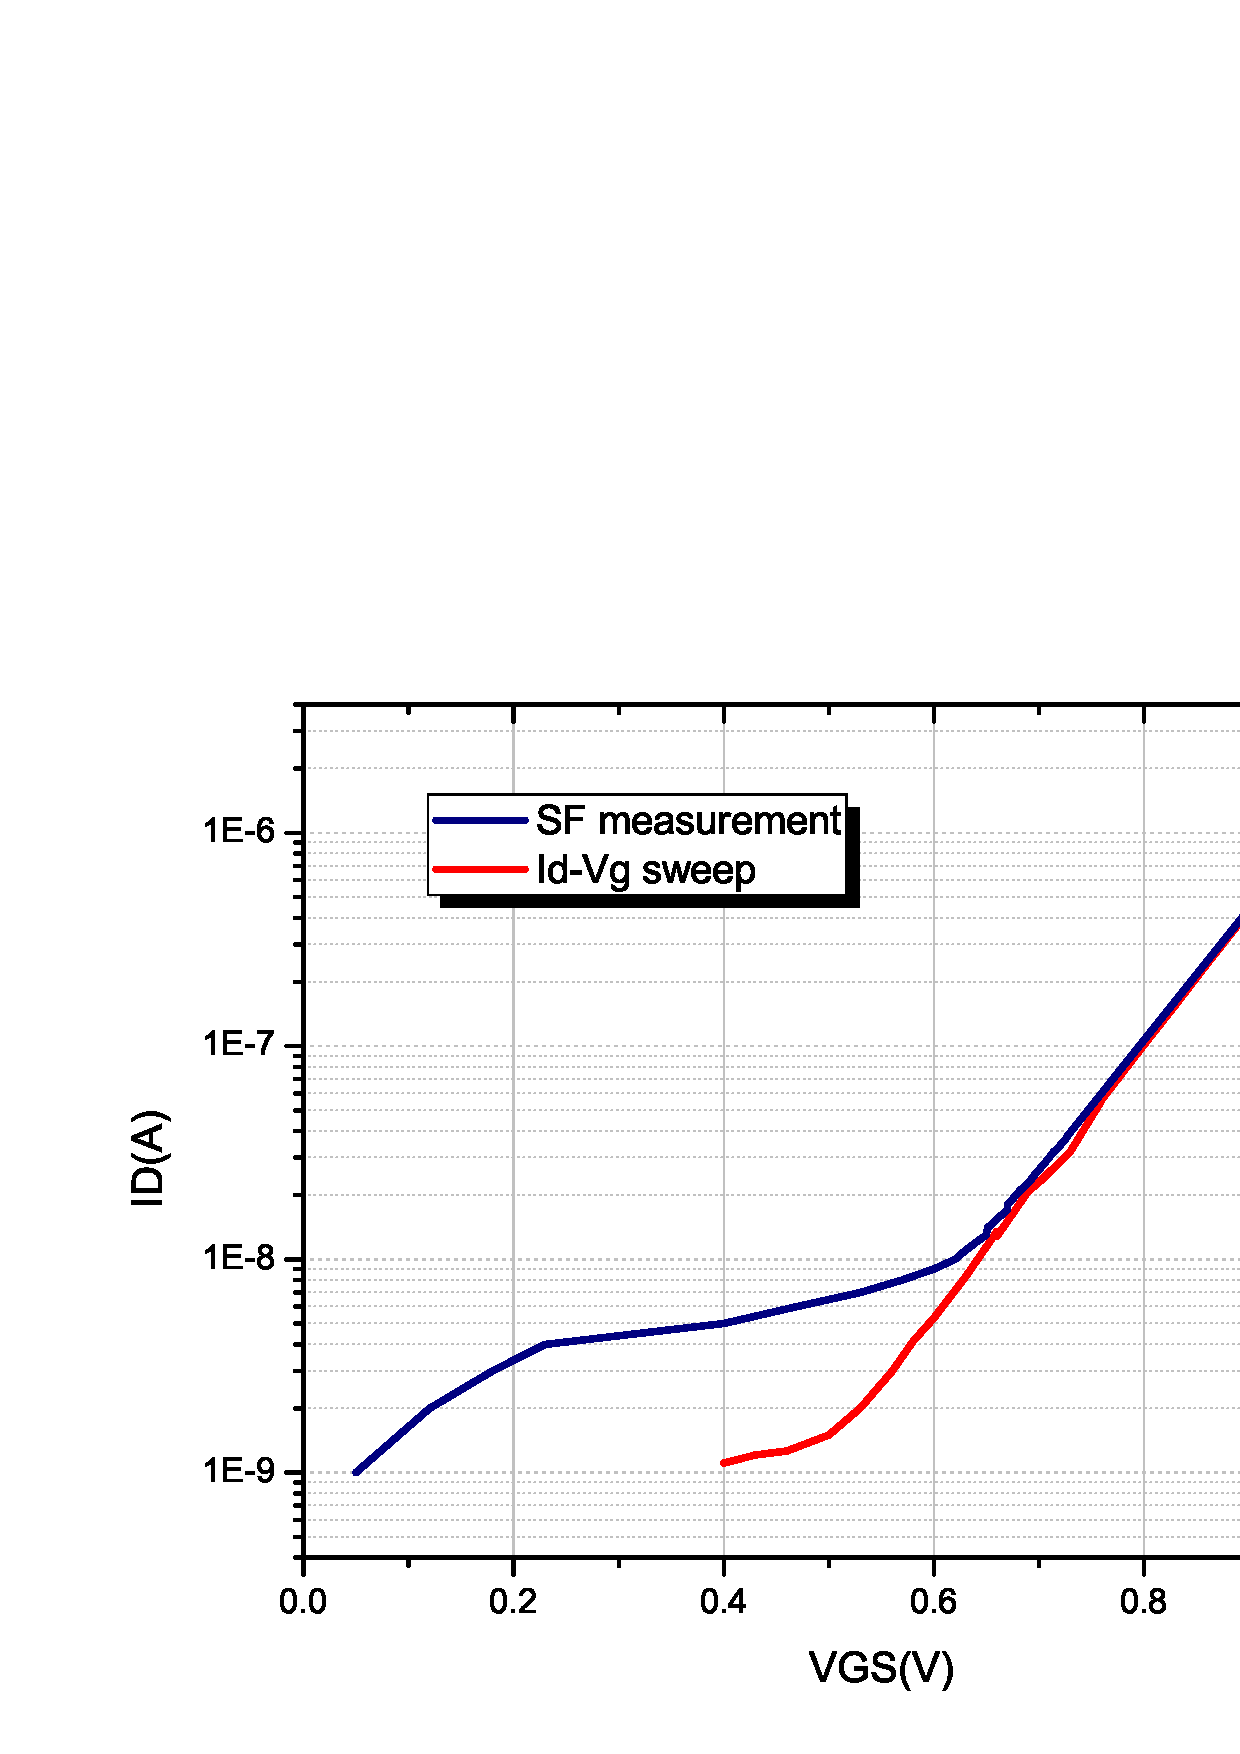
\includegraphics[width=0.8\textwidth]{images/chapter4/SF.png}
    \caption{The measuremet result (``SF\_measurement'') compares with the direct $I_D$-$V_G$ sweep (``Id-Vg sweep'').}
    \label{fig:SF_result}
\end{figure}

\begin{figure}[!htbp]
   \centering
   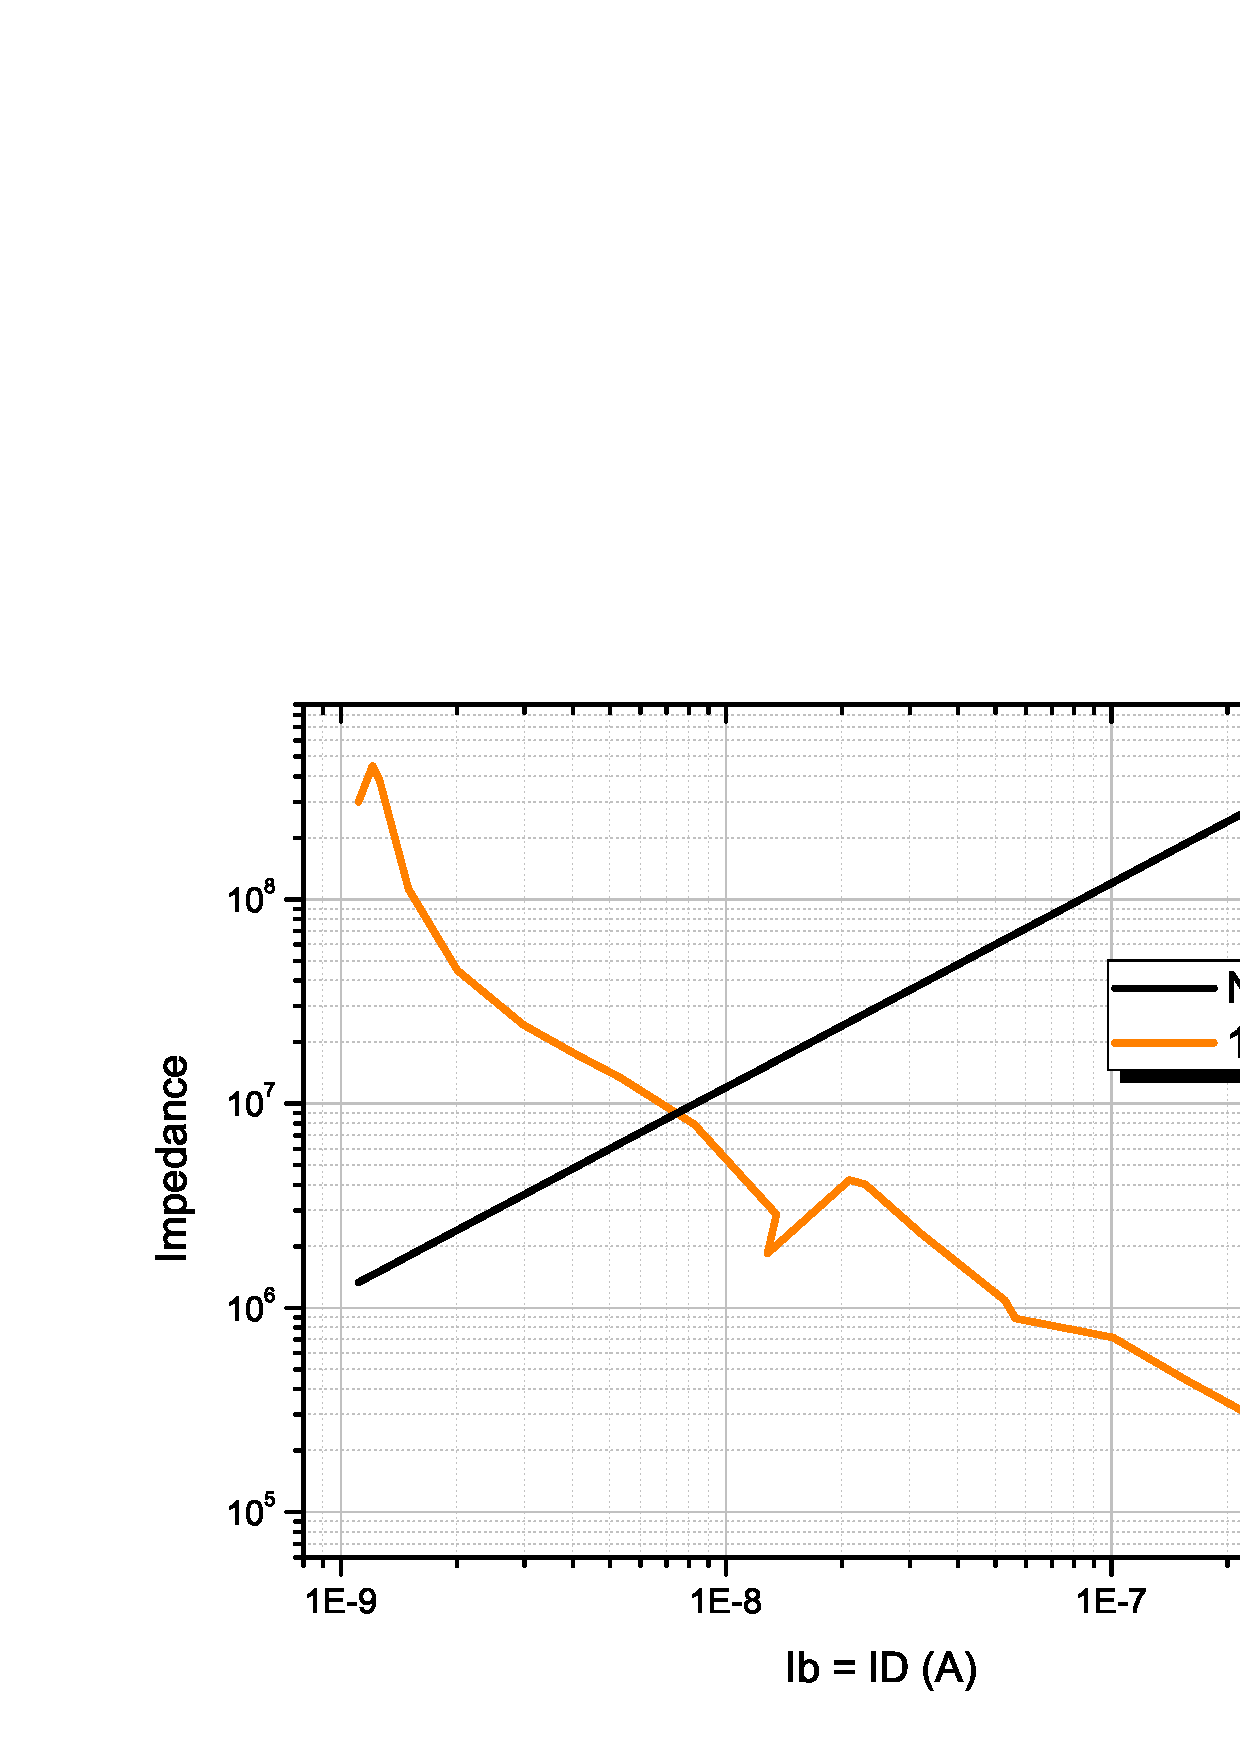
\includegraphics[width=0.8\textwidth]{../images/chapter4/SF_impedance.png}
   \caption{Input impedance of transistor (``1/gm'') and output impedance of Ib circuit (``Rs''). The former is found by the derivative of $I_D$ of $V_{Gs}$. The latter is obtained by Eq.\ref{eq:rcs2_again}.}
   \label{fig:SF_imp}
\end{figure}

Fig.\ref{fig:SF_imp} proves that the $R_s$ is close to the input impedance of transistor around $I_D = 10n A$, where the $g_m$ of transistor is around $1 / 10M$.
The result means that we overestimate the $I_b$.

Overall, the constant current method is feasible.
What one needs to noticed when applying the constant current method is the impedance matching.
In source follower structure, its current input impedance varies with the bias current.
The varying range effect the dynamic range and need more design concern.


